\documentclass[preprint,12pt,aps,pra,showkeys,amsmath,amssymb,superscriptaddress,floatfix]{revtex4-2}
\usepackage[T1]{fontenc}
\usepackage[utf8]{inputenc}
\usepackage{amsmath,amssymb,amsthm,mathtools,mathrsfs}
\usepackage{microtype,booktabs,enumitem}
\usepackage{xcolor,tikz,etoolbox}
\usepackage[skins,breakable]{tcolorbox}
\usepackage{needspace}
% Keep diagram geometry independent of REVTeX preprint body spacing.
\AtBeginEnvironment{tikzpicture}{\linespread{1}\selectfont}
\usetikzlibrary{arrows.meta,positioning,calc,fit,decorations.pathreplacing}
\usepackage{graphicx}
\usepackage{hyperref}

\definecolor{MMBlue}{RGB}{0,82,155}
\definecolor{MMOrange}{RGB}{200,80,0}
\tikzset{
 mmnode/.style={draw=MMBlue,rounded corners=2pt,fill=MMBlue!4,align=left,execute at begin node={\raggedright},text width=5cm,font=\fontsize{10}{12}\selectfont,inner sep=6pt},
 mmimport/.style={mmnode,draw=black!65,fill=black!4},
 mmcandidate/.style={mmnode,draw=MMOrange,dashed,fill=MMOrange!5},
 mmrejected/.style={mmnode,draw=black,densely dotted,fill=black!8},
 mmproof/.style={->,thick,MMBlue},
 mmflow/.style={->,semithick,black!70},
 mmrepair/.style={->,dashed,thick,MMOrange},
 mmcandidatearrow/.style={->,dashed,semithick,MMOrange},
 mmnote/.style={font=\scriptsize,fill=white,inner sep=2pt,align=center}}

\usepackage[section]{placeins}
\setlength{\emergencystretch}{3em}
\setlist{itemsep=3pt,topsep=4pt}
\newtheorem{theorem}{Theorem}[section]
\newtheorem{proposition}[theorem]{Proposition}
\newtheorem{lemma}[theorem]{Lemma}
\newtheorem{corollary}[theorem]{Corollary}
\theoremstyle{definition}
\newtheorem{definition}[theorem]{Definition}
\newtheorem{example}[theorem]{Example}
\theoremstyle{remark}
\newtheorem{remark}[theorem]{Remark}
% Avoid isolated statement headings and single-line paragraph fragments.
\BeforeBeginEnvironment{theorem}{\Needspace{6\baselineskip}}
\BeforeBeginEnvironment{definition}{\Needspace{5\baselineskip}}
\BeforeBeginEnvironment{proposition}{\Needspace{5\baselineskip}}
\BeforeBeginEnvironment{lemma}{\Needspace{5\baselineskip}}
\BeforeBeginEnvironment{corollary}{\Needspace{5\baselineskip}}
\clubpenalty=5000
\widowpenalty=5000
\newcommand{\R}{\mathbb R}\newcommand{\Z}{\mathbb Z}\newcommand{\N}{\mathbb N}
\newcommand{\Pa}{\operatorname{Pa}}\newcommand{\Desc}{\operatorname{Desc}}
\newcommand{\cl}{\operatorname{cl}}\newcommand{\cost}{\operatorname{cost}}
\newcommand{\status}{\operatorname{status}}
% Faculty cards: a visual rail groups the five faculties within one agent.
% The rail has no arrowhead and does not represent a proof dependency.
\newcommand{\mmfacultybadge}[1]{%
 \node[circle,draw=MMBlue,line width=1pt,fill=white,
 minimum size=7mm,inner sep=0pt,font=\sffamily\small\bfseries,text=MMBlue]
 at ([xshift=15pt,yshift=-15pt]frame.north west) {#1};}
\newcommand{\mmfacultyrail}{%
 \draw[MMBlue!80,line width=1pt]
 ([xshift=15pt,yshift=2pt]frame.north west)--
 ([xshift=15pt,yshift=-2pt]frame.south west);}
\newtcolorbox{mmfacultybox}[2]{enhanced,breakable,
 colback=MMBlue!4,colframe=MMBlue!4,boxrule=0pt,arc=3pt,
 left=39pt,right=9pt,top=4pt,bottom=4pt,
 before skip=2pt,after skip=2pt,
 fontupper=\small\linespread{1.1}\selectfont,
 overlay unbroken={\mmfacultyrail\mmfacultybadge{#1}},
 overlay first={\mmfacultyrail\mmfacultybadge{#1}},
 overlay middle={\mmfacultyrail},overlay last={\mmfacultyrail}}
\newcommand{\mmfaculty}[3]{%
 \begin{mmfacultybox}{#1}{#2}
 {\sffamily\bfseries\color{MMBlue}#2}\par\smallskip #3
 \end{mmfacultybox}}
\newcommand{\agent}[9]{%
 \Needspace{8\baselineskip}
 \subsubsection{#1}
 \noindent\textbf{Object.} #2\par
 \noindent\textbf{Role.} #3\par\smallskip
 \mmfaculty{E}{Ego}{#4}
 \mmfaculty{M}{Memory}{#5}
 \mmfaculty{I}{Intellect}{#6}
 \mmfaculty{S}{Sense}{#7}
 \mmfaculty{A}{Action}{#8}
 \smallskip\noindent #9\par}

\usepackage{longtable,array,calc}
\providecommand{\tightlist}{\setlength{\itemsep}{2pt}\setlength{\parskip}{0pt}}
\makeatletter
\def\frontmatter@abstract@produce{\par\addvspace{\frontmatter@preabstractspace}%
\begingroup\prep@absbox\unvbox\absbox\post@absbox\endgroup
\addvspace{\frontmatter@postabstractspace}}
\makeatother
\newcommand{\field}[2]{\par\smallskip\noindent\textbf{#1.} #2\par}
\setlength{\emergencystretch}{5em}
\AtBeginEnvironment{verbatim}{\small\linespread{1.0}\selectfont}


\hypersetup{colorlinks=true,linkcolor=MMBlue,urlcolor=MMBlue,pdfauthor={Dibakar Sigdel}}

\begin{document}

\title{Fourier Orthogonality and Bessel's Inequality\\[4pt]\large An End-to-End Meta-Math Walkthrough}

\author{Dibakar Sigdel}

\affiliation{Mindverse Computing LLC, Lynnwood, WA 98087, USA}

\date{October 2026}

\begin{abstract}

A complete authored walkthrough of fourier orthogonality and bessel's
inequality, with explicit mathematical contracts, local verification
gates, and reusable exports. The report presents the target theorem,
declared imports, a dependency graph, five-faculty node contracts, a
continuous proof, a worked example, and a hypothesis-repair audit. It is
an authored mathematical exposition, not a deployed-agent transcript or
a formal proof-assistant certificate.

\end{abstract}\maketitle\linespread{1.12}\selectfont

\noindent\textbf{HA-01 / Harmonic Analysis / Report v1}

\section{Target and import contract}

\begin{theorem}

On \(\mathbb T=\mathbb R/(2\pi\mathbb Z)\) with measure \(dx/(2\pi)\),
prove \(e^{inx}\) form an orthonormal system. For
\(f\in L^2(\mathbb T)\) and \(c_n=\int f(x)e^{-inx}\,dx/(2\pi)\), prove
\(\sum_{n\in\mathbb Z}|c_n|^2\le\|f\|_2^2\).

\end{theorem}

\subsection{Foundations and permitted imports}

Use normalized measure \(dx/(2\pi )\) on T. The complex inner product is
\(\langle f,g\rangle =\int f\) \(\operatorname{conj} (g)\), linear in
the first argument. \(L^{2}\) functions on this probability space are
\(L^{1}\) by Cauchy--Schwarz, so coefficients are defined. Only finite
orthogonal projection and monotone limits of nonnegative sums are
needed.

\clearpage\section{Node interaction workflow}

\begin{center}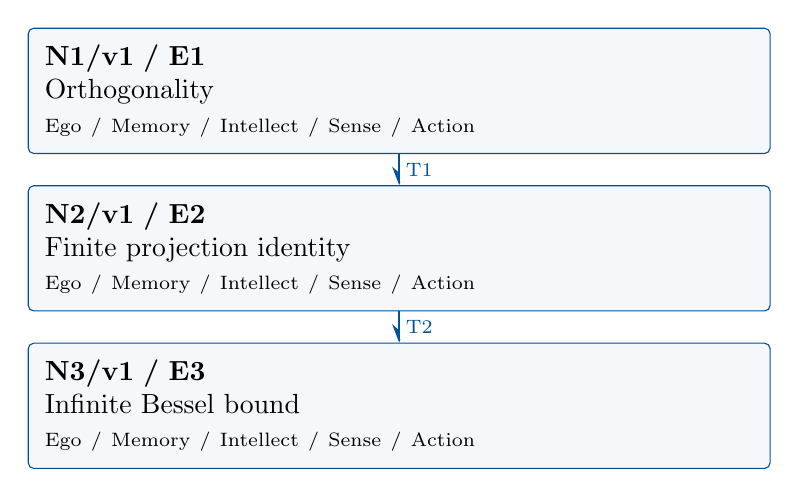
\begin{tikzpicture}[>=Stealth,x=1cm,y=1cm]

\node[mmnode,text width=9cm,minimum height=1.25cm] (N1) at (0,0.0) {\textbf{N1/v1 / E1}\\Orthogonality\\{\scriptsize Ego / Memory / Intellect / Sense / Action}};

\node[mmnode,text width=9cm,minimum height=1.25cm] (N2) at (0,-2.0) {\textbf{N2/v1 / E2}\\Finite projection identity\\{\scriptsize Ego / Memory / Intellect / Sense / Action}};

\node[mmnode,text width=9cm,minimum height=1.25cm] (N3) at (0,-4.0) {\textbf{N3/v1 / E3}\\Infinite Bessel bound\\{\scriptsize Ego / Memory / Intellect / Sense / Action}};

\draw[mmproof] (N1.south) -- node[mmnote,right] {T1} (N2.north);

\draw[mmproof] (N2.south) -- node[mmnote,right] {T2} (N3.north);

\end{tikzpicture}\end{center}

Each box is one mathematical agent containing all five faculties. Blue
arrows carry the versioned exports listed below. The layout gives a
reading order; only drawn arrows assert dependencies. Diagnostic repair
is separate from the proof DAG.

\subsection{Versioned evidence-transfer ledger}

\begingroup\small\linespread{1.05}\selectfont

\Needspace{5\baselineskip}\field{T1: N1/E1/v1 to N2}{\(\langle e_n,e_m\rangle =\delta _nm\).}

\field{Receiving activity}{N2: Finite projection identity}

\field{Compatibility}{Use the same mathematical objects and hypotheses as the source export.
Receiving contract: Finite set \(F\subset Z\);
\(c_n=\langle f,e_n\rangle\); prior exports E1/v1}

\Needspace{5\baselineskip}\field{T2: N2/E2/v1 to N3}{Exact finite projection identity and finite Bessel bound.}

\field{Receiving activity}{N3: Infinite Bessel bound}

\field{Compatibility}{Use the same mathematical objects and hypotheses as the source export.
Receiving contract: Bounds for \(F=\{-N,\ldots ,N\}\); prior exports
E2/v1}

\endgroup

\clearpage\section{Agent roles and five-faculty activities}\begingroup\small\linespread{1.05}\selectfont\setlist{itemsep=1pt,topsep=2pt}

\subsection{N1/v1: Orthogonality}

\field{Object and role}{Integrate frequency differences.}

\field{Inputs}{\(e_n(x)=e^{inx}\); normalized measure; foundational imports stated in
§1}

\mmfaculty{E}{Ego}{Own E1/v1: \(\langle e_n,e_m\rangle =\delta _nm\).}

\mmfaculty{M}{Memory}{Retain \(e_n(x)=e^{inx}\); normalized measure; foundational imports
stated in §1; keep their assumptions and versions attached.}

\mmfaculty{I}{Intellect}{Integrate frequency differences.}

\mmfaculty{S}{Sense}{A different measure would change the norms and coefficients.}

\mmfaculty{A}{Action}{Carry out the numbered deductions and publish E1/v1 together with its
hypotheses and proof location.}

\smallskip\noindent\textbf{Numbered mathematical activities}

\begin{enumerate}[label=N1.\arabic*,leftmargin=3.4em]

\item For \(m=n\), \(\langle e_n,e_m\rangle =\int 1\) \(dx/(2\pi )=1\).

\item For \(m\ne n\), integrating \(e^{i(n-m)x}\) \(over[-\pi ,\pi ]\) gives
zero since its endpoint values agree.

\item Thus the exponentials are orthonormal.

\end{enumerate}

\field{Export E1/v1}{\(\langle e_n,e_m\rangle =\delta _nm\).}

\field{Acceptance gate}{A different measure would change the norms and coefficients. Publish
only after checking every displayed deduction.}

\field{Targeted repair}{If the check fails, revise N1: A different measure would change the
norms and coefficients. Recheck dependent nodes N2, N3.}

\clearpage

\subsection{N2/v1: Finite projection identity}

\field{Object and role}{Use an orthogonal residual.}

\field{Inputs}{Finite set \(F\subset Z\); \(c_n=\langle f,e_n\rangle\); prior exports
E1/v1}

\mmfaculty{E}{Ego}{Own E2/v1: Exact finite projection identity and finite Bessel bound.}

\mmfaculty{M}{Memory}{Retain Finite set \(F\subset Z\); \(c_n=\langle f,e_n\rangle\); prior
exports E1/v1; keep their assumptions and versions attached.}

\mmfaculty{I}{Intellect}{Use an orthogonal residual.}

\mmfaculty{S}{Sense}{Orthonormality alone does not yet imply completeness.}

\mmfaculty{A}{Action}{Carry out the numbered deductions and publish E2/v1 together with its
hypotheses and proof location.}

\smallskip\noindent\textbf{Numbered mathematical activities}

\begin{enumerate}[label=N2.\arabic*,leftmargin=3.4em]

\item Let \(P_F\) \(f=\sum _{n\in F}c_ne_n\).

\item Orthogonality gives \(\langle f-P_F\) \(f,e_m\rangle =0\) for \(m\in F\)
and \(\Vert P_F\) \(f\Vert ^{2}=\sum _{n\in F}|c_n|^{2}\).

\item Expand the norm of \(f=P_F\) \(f+(f-P_F\) f); the cross term vanishes,
so \(\Vert f\Vert ^{2}=\sum _{n\in F}|c_n|^{2}+\Vert f-P_F\)
\(f\Vert ^{2}\).

\item Therefore every finite coefficient sum is at most \(\Vert f\Vert ^{2}\).

\end{enumerate}

\field{Export E2/v1}{Exact finite projection identity and finite Bessel bound.}

\field{Acceptance gate}{Orthonormality alone does not yet imply completeness. Publish only after
checking every displayed deduction.}

\field{Targeted repair}{If the check fails, revise N2: Orthonormality alone does not yet imply
completeness. Recheck dependent nodes N3.}

\clearpage

\subsection{N3/v1: Infinite Bessel bound}

\field{Object and role}{Pass to a monotone nonnegative series.}

\field{Inputs}{Bounds for \(F=\{-N,\ldots ,N\}\); prior exports E2/v1}

\mmfaculty{E}{Ego}{Own E3/v1: Bessel's inequality under the fixed normalization.}

\mmfaculty{M}{Memory}{Retain Bounds for \(F=\{-N,\ldots ,N\}\); prior exports E2/v1; keep
their assumptions and versions attached.}

\mmfaculty{I}{Intellect}{Pass to a monotone nonnegative series.}

\mmfaculty{S}{Sense}{Do not replace the inequality by equality before proving density.}

\mmfaculty{A}{Action}{Carry out the numbered deductions and publish E3/v1 together with its
hypotheses and proof location.}

\smallskip\noindent\textbf{Numbered mathematical activities}

\begin{enumerate}[label=N3.\arabic*,leftmargin=3.4em]

\item The sums \(\sum _{|n|\le N}|c_n|^{2}\) increase and are bounded above by
\(\Vert f\Vert ^{2}\).

\item Their limit is the nonnegative bilateral series, proving
\(\sum _Z|c_n|^{2}\le \Vert f\Vert ^{2}\).

\item No convergence of Fourier partial sums to f has been assumed; equality
requires the density bridge in HA-03.

\end{enumerate}

\field{Export E3/v1}{Bessel's inequality under the fixed normalization.}

\field{Acceptance gate}{Do not replace the inequality by equality before proving density.
Publish only after checking every displayed deduction.}

\field{Targeted repair}{If the check fails, revise N3: Do not replace the inequality by equality
before proving density. Withhold this terminal result until its gate
passes.}

\endgroup\clearpage\section{Continuous mathematical proof}\label{sec:proof}

Read these steps in order as one proof; the diagram is optional.
Numbered activities identify the specific constructions and deductions
owned by each node.

\subsection{§4.N1 --- Orthogonality}\label{n1-orthogonality}

\begin{enumerate}
\def\labelenumi{\arabic{enumi}.}
\item
  For \(m=n\), \(\langle e_n,e_m\rangle =\int 1\) \(dx/(2\pi )=1\).
\item
  For \(m\ne n\), integrating \(e^{i(n-m)x}\) \(over[-\pi ,\pi ]\) gives
  zero since its endpoint values agree.
\item
  Thus the exponentials are orthonormal.
\end{enumerate}

\subsection{§4.N2 --- Finite projection
identity}\label{n2-finite-projection-identity}

\begin{enumerate}
\def\labelenumi{\arabic{enumi}.}
\item
  Let \(P_F\) \(f=\sum _{n\in F}c_ne_n\).
\item
  Orthogonality gives \(\langle f-P_F\) \(f,e_m\rangle =0\) for
  \(m\in F\) and \(\Vert P_F\) \(f\Vert ^{2}=\sum _{n\in F}|c_n|^{2}\).
\item
  Expand the norm of \(f=P_F\) \(f+(f-P_F\) f); the cross term vanishes,
  so \(\Vert f\Vert ^{2}=\sum _{n\in F}|c_n|^{2}+\Vert f-P_F\)
  \(f\Vert ^{2}\).
\item
  Therefore every finite coefficient sum is at most
  \(\Vert f\Vert ^{2}\).
\end{enumerate}

\subsection{§4.N3 --- Infinite Bessel
bound}\label{n3-infinite-bessel-bound}

\begin{enumerate}
\def\labelenumi{\arabic{enumi}.}
\item
  The sums \(\sum _{|n|\le N}|c_n|^{2}\) increase and are bounded above
  by \(\Vert f\Vert ^{2}\).
\item
  Their limit is the nonnegative bilateral series, proving
  \(\sum _Z|c_n|^{2}\le \Vert f\Vert ^{2}\).
\item
  No convergence of Fourier partial sums to f has been assumed; equality
  requires the density bridge in HA-03.
\end{enumerate}

\hfill$\square$

\section{Worked orchestration}

For \(f=2+3cosx\), \(c_{0}=2\) and \(c_{\pm 1}=3/2\), with all other
coefficients 0. Thus the sum is \(4+2\cdot 9/4=17/2\). Direct
integration \(of|f|^{2}\) under normalized measure gives 17/2,
illustrating the finite orthogonal decomposition.

\subsection{Boundary and hypothesis audit}

In a general Hilbert space, an orthonormal system need not span the
space: a single vector in \(R^{2}\) misses its perpendicular direction.
Sense blocks a candidate equality export from the Bessel proof; Fourier
completeness must be supplied separately.

\section{Illustrative failure and repair}

The following is an authored diagnostic scenario. Changed assumptions
define a new contract; they do not retroactively prove the original
statement.

\subsection{Failure and correction}
This is an authored teaching trace, not a recorded agent run.

\begin{enumerate}
\def\labelenumi{\arabic{enumi}.}
\tightlist
\item
  \textbf{Ego \(\to\) Memory:} register the §1 theorem, imports, and
  requested exports before beginning the proof.
\item
  \textbf{Intellect \(\to\) Action:} choose the bridges in §3 and carry
  out the numbered activities in §4; transmit only established E-exports
  along the §2 DAG.
\item
  \textbf{Sense \(\to\) responsible node:} test the specific
  boundary/failure in §5 and the node's individual audit. A failing
  candidate is withheld; downstream nodes may not use it.
\item
  \textbf{Memory + Intellect:} identify whether the error is an omitted
  condition, an invalid inference, or an attempted extension beyond the
  theorem. Restore the exact contract or explicitly state a different
  one.
\item
  \textbf{Action:} redo the affected mathematical activity using the
  repaired condition or inference. Recheck consuming nodes, rather than
  feeding their conclusions back as premises.
\item
  \textbf{Ego:} publish only the supported export with its assumptions
  and proof location. A hypothetical revised export is v2; the written
  proof here is the v1 exposition, not a claim that this repair was
  executed.
\end{enumerate}

\subsection{Hypothesis boundary}
In a general Hilbert space, an orthonormal system need not span the
space: a single vector in \(R^{2}\) misses its perpendicular direction.
Sense blocks a candidate equality export from the Bessel proof; Fourier
completeness must be supplied separately.

\subsection{Version and recheck}
Treat any changed assumption as a new contract. Recheck the revised
export and all of its descendants. A backward diagnostic never
establishes an earlier theorem. This is an authored teaching trace, not
an execution log.

\par\medskip\begingroup\small\linespread{1.0}\selectfont\noindent\textbf{Provenance.} This authored proof is complete relative to its declared imports. Reuse
each export with its assumptions, proof, and version. The original
Markdown remains available for comparison.
\par\endgroup

\end{document}
